\documentclass[usenames,dvipsnames,tikz]{standalone}
\usetikzlibrary{shapes.geometric}
\usepackage{xcolor}
\colorlet{tBlue}{RoyalBlue!35!Cerulean}
\colorlet{tRed}{Red}
\usepackage{tikz}
\usepackage{standalone}
\begin{document}	
	
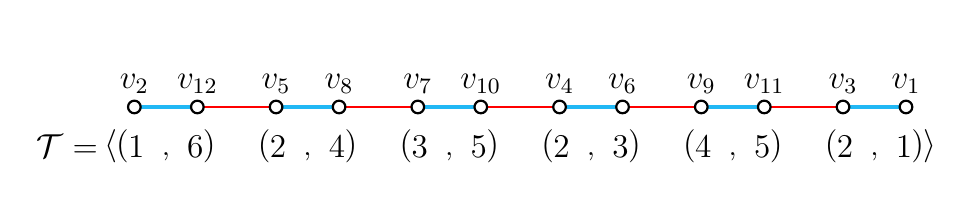
\begin{tikzpicture}
%\draw [help lines] (-1,-1) grid (14, 6);

\draw [white] (1,4) -- (10.8,4);

\draw [ultra thick, tBlue] (1,3) -- (1.8,3);
\draw [ultra thick, tBlue] (2.8,3) -- (3.6,3);
\draw [ultra thick, tBlue] (4.6,3) -- (5.4,3);
\draw [ultra thick, tBlue] (6.4,3) -- (7.2,3);
\draw [ultra thick, tBlue] (8.2,3) -- (9,3);
\draw [ultra thick, tBlue] (10,3) -- (10.8,3);

\draw [tRed] (1.8,3) -- (2.8,3);
\draw [tRed] (3.6,3) -- (4.6,3);
\draw [tRed] (5.4,3) -- (6.4,3);
\draw [tRed] (7.2,3) -- (8.2,3);
\draw [tRed] (9,3) -- (10,3);

\draw [fill=white, thick] (1,3) circle [radius = 0.08];
\draw [fill=white, thick] (1.8,3) circle [radius = 0.08];
\draw [fill=white, thick] (2.8,3) circle [radius = 0.08];
\draw [fill=white, thick] (3.6,3) circle [radius = 0.08];
\draw [fill=white, thick] (4.6,3) circle [radius = 0.08];
\draw [fill=white, thick] (5.4,3) circle [radius = 0.08];
\draw [fill=white, thick] (6.4,3) circle [radius = 0.08];
\draw [fill=white, thick] (7.2,3) circle [radius = 0.08];
\draw [fill=white, thick] (8.2,3) circle [radius = 0.08];
\draw [fill=white, thick] (9,3) circle [radius = 0.08];
\draw [fill=white, thick] (10,3) circle [radius = 0.08];
\draw [fill=white, thick] (10.8,3) circle [radius = 0.08];

\node [above] at (1,3.05) {\large{$v_2$}};
\node [above] at (1.8,3.05) {\large{$v_{12}$}};
\node [above] at (2.8,3.05) {\large{$v_5$}};
\node [above] at (3.6,3.05) {\large{$v_8$}};
\node [above] at (4.6,3.05) {\large{$v_7$}};
\node [above] at (5.4,3.05) {\large{$v_{10}$}};
\node [above] at (6.4,3.05) {\large{$v_4$}};
\node [above] at (7.2,3.05) {\large{$v_6$}};
\node [above] at (8.2,3.05) {\large{$v_9$}};
\node [above] at (9,3.05) {\large{$v_{11}$}};
\node [above] at (10,3.05) {\large{$v_3$}};
\node [above] at (10.8,3.05) {\large{$v_1$}};

\node at (1.025,2.5) {\large{1}};
\node at (1.775,2.5) {\large{6}};
\node at (2.825,2.5) {\large{2}};
\node at (3.575,2.5) {\large{4}};
\node at (4.625,2.5) {\large{3}};
\node at (5.375,2.5) {\large{5}};
\node at (6.425,2.5) {\large{2}};
\node at (7.175,2.5) {\large{3}};
\node at (8.225,2.5) {\large{4}};
\node at (8.975,2.5) {\large{5}};
\node at (10.025,2.5) {\large{2}};
\node at (10.775,2.5) {\large{1}};

\node at (1.4,2.37) {,};
%\node at (2.5,2.37) {,};
\node at (3.2,2.37) {,};
%\node at (4.5,2.37) {,};
\node at (5,2.37) {,};
%\node at (6.5,2.37) {,};
\node at (6.8,2.37) {,};
%\node at (8.5,2.37) {,};
\node at (8.6,2.37) {,};
%\node at (10.5,2.37) {,};
\node at (10.4,2.37) {,};

\node at (0.85,2.5) {\large{(}};
\node at (1.95,2.5) {\large{)}};
\node at (2.65,2.5) {\large{(}};
\node at (3.75,2.5) {\large{)}};
\node at (4.45,2.5) {\large{(}};
\node at (5.55,2.5) {\large{)}};
\node at (6.25,2.5) {\large{(}};
\node at (7.35,2.5) {\large{)}};
\node at (8.05,2.5) {\large{(}};
\node at (9.15,2.5) {\large{)}};
\node at (9.85,2.5) {\large{(}};
\node at (10.95,2.5) {\large{)}};

\node at (0.7, 2.5) {\large{$\langle$}};
\node at (11.1, 2.5) {\large{$\rangle$}};

\node at (0.15, 2.5) {\large{$\mathcal{T} =$}};

\end{tikzpicture}
	
\end{document}
